\chapter{Modelle}
\section{Szenarios}
\subsection{Überwachung und Messung an einem Versuchsaufbau}
Angenommen jemand hat einen Versuchsaufbau mit mehreren Temperatur Sensoren des gleichen Types aufgebaut und will damit seine Wohnung, über die Dauer einer Woche, überwachen. Der Aufbau ist relativ schnell bewälltigt und das größte Problem ist die Flut an Daten die bewältigt werden muss, wenn jede Minute ein Wert pro Sensor gespeichert werden soll. Darüber hinaus sollen die Daten so gespeichert werden, das eine spätere Auswertung, evtl. auch durch Dritte, nach gängigen Normel vorgenommen werden kann. Der Nutzer hat in seinem beruflichen Umfeld bereits Erfahrungen mit Elektrotechnik gesammelt und ist geübt im Umgang mit Computern und der Bedienung von Anwendungen.

Der Aufbau ist abgeschlossen und er sucht nur noch nach einer Software die seinen Bedürfnissen entspricht. Hier kommt die zu entwickelnde Software ins Spiel. Er startet die Software und konfiguriert  seine Messung mit Hilfe des Wizards nach seinen Vorstellungen. Er will das die Werte nicht nur generisch "A1", "`A2"' und so weiter heißen, sondern entsprechender des Raumes in dem sich der Sensor befindet beschriftet werden. Sofort sieht er in dem Wizard diese Option und trägt die Beschriftung der Pins in die vorgesehenen Textboxen ein. Da die Sensoren nur ein analoges Signal im Rahmen von 0 bis 5 Volt ausgeben und dieses Signal noch in Grad Celsius umgewandelt werden muss trägt er zu jedem Pin noch die entsprechende Übertragungsfunktion ein. Nachdem dies geschehen ist geht er in dem Wizard eine Schritt weiter und bekommt die Möglichkeit die digitalen Pins des Arduinos zu Steuern. Er entscheidet sich gegen die Nutzung. Es sollen lediglich Daten gemessen und geloggt werden. Auf der letzten Seite des Wizards bekommt er die Optionen zu Einrichtung des \acrshort{CSV}-Loggers. Da er die Software auf einer deutschsprachigen Maschine betreibt und die anschließende Auswertung auch in einer deutschsprachigen Tabelenbearbeitungssoftware geschehen wird, gibt er an, dass entsprechende Tausendertrenner und ähnliches verwendet werden sollen. Der Wizard hat ihm allerdings auf Grund der verwendeten System-Einstellungen diesen Vorschlag bereits unterbreitet. Der Nutzer gibt nur noch an das er sowohl die umgerechneten Temperaturen und die Spannungswerte in dem Log hinterlegt haben möchte. 

Nach dem die Konfiguration abgeschlossen ist, muss noch der Arduino-Sketch mittels der Arduino eigenen IDE installiert werden. Ist dies erfolgt kann die Messung beginnen. Der Nutzer bekommt nun in Echtzeit die gemessenen Werte angezeigt. Er kann selektiv nur einen oder mehrere Werte anzeigen lassen und zwischen den Spannungswerten und den umgerechneten Werten auswählen. Zusätzlich kann er sich noch eine Tendenz einblenden lassen, um etwa zu sehen wann und wo er vergessen hat ein Fenster zu schließen und somit der Raum auskühlt. 

Nun da die Messung läuft kann er sich anderen Dingen zu wenden und ggf. ab und zu nachschauen ob es interessante Veränderungen in den gemessen Werten gibt.
Nach Ablauf der einen Woche beendet er die Messung und kann nun die Werte mit Hilfe einer anderen Software genauer überprüfen.
\subsection{Steuerung und Messung an einem Versuchsaufbau}
\section{Use case model}
Dieses Use case Diagramm zeigt die dem Nutzer zu Verfügung stehen Optionen.
\begin{figure}[H]
 \centering
 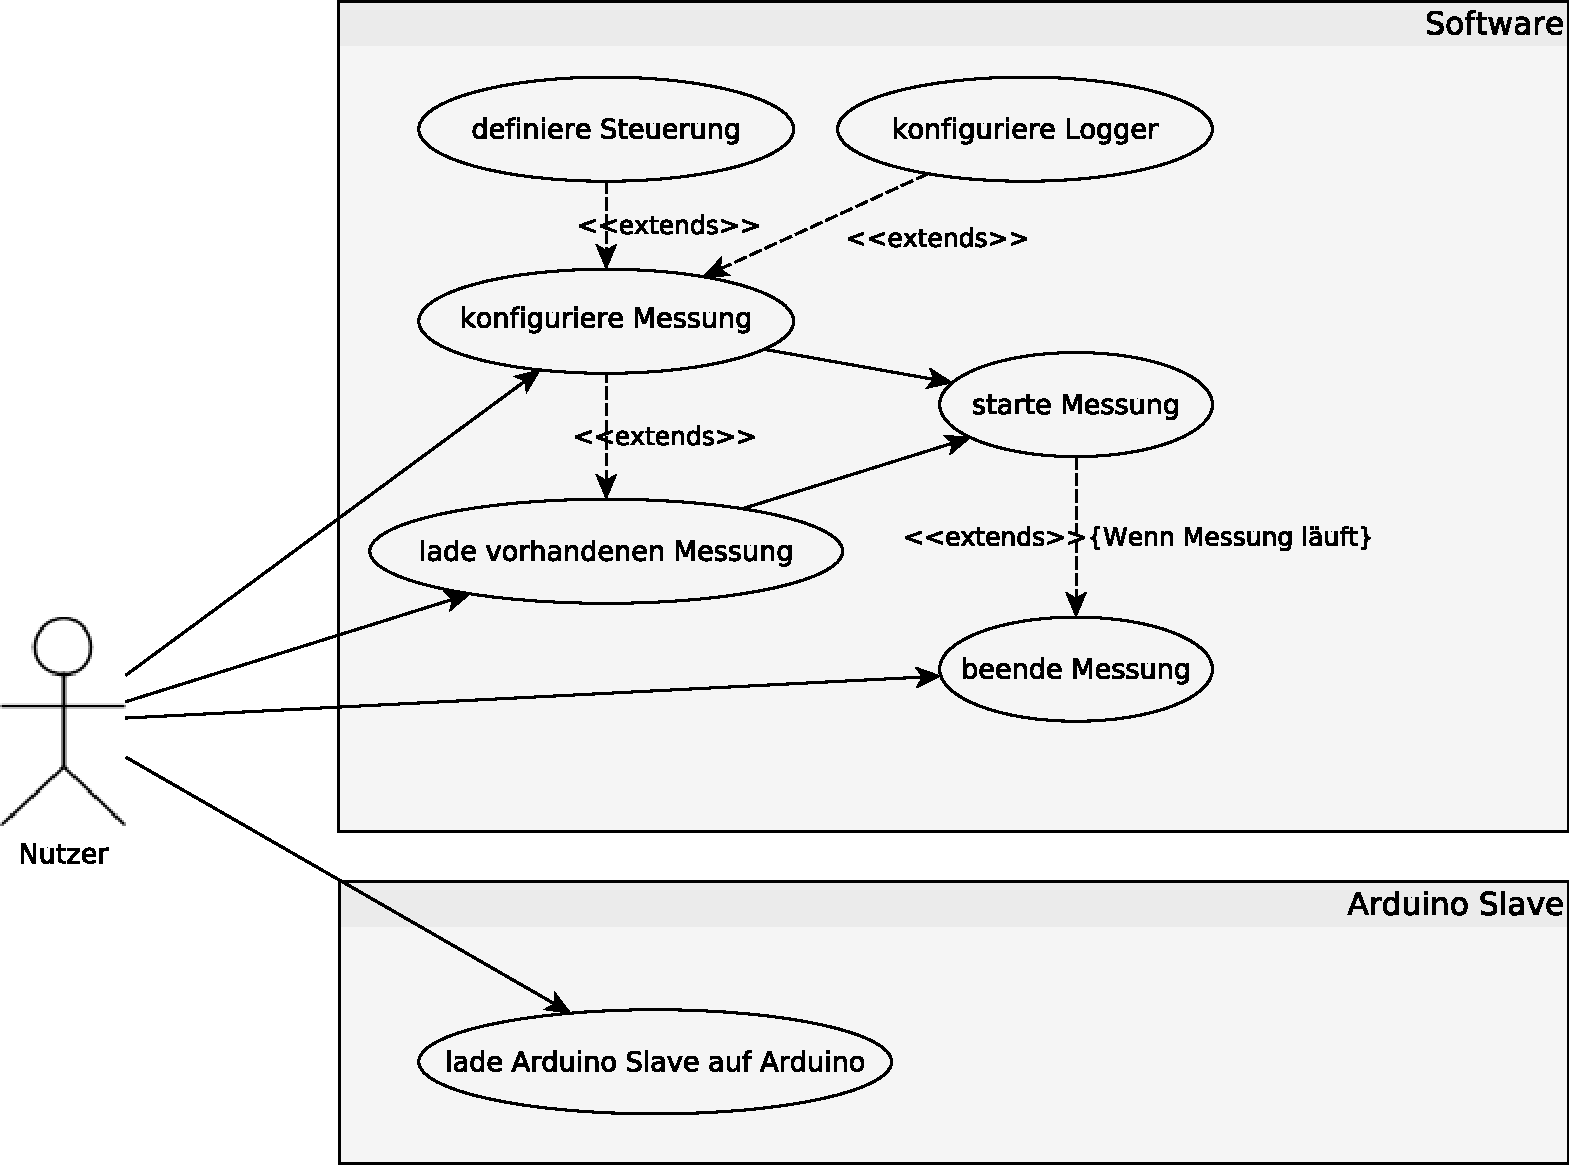
\includegraphics[width=\textwidth, keepaspectratio=true]{../Diagramme/BachelorUseCase1.pdf}
\end{figure}

%\section{Analysis object model}
%\section{Dynamic model}
\section{Flowchart}
Dieses Flowchart zeigt die notwendigsten Schritte, die von der Software und dem Nutzer unternommen werden müssen um eine erfolgreiche Messung durch führen zu können. 
\begin{figure}[H]
 \centering
 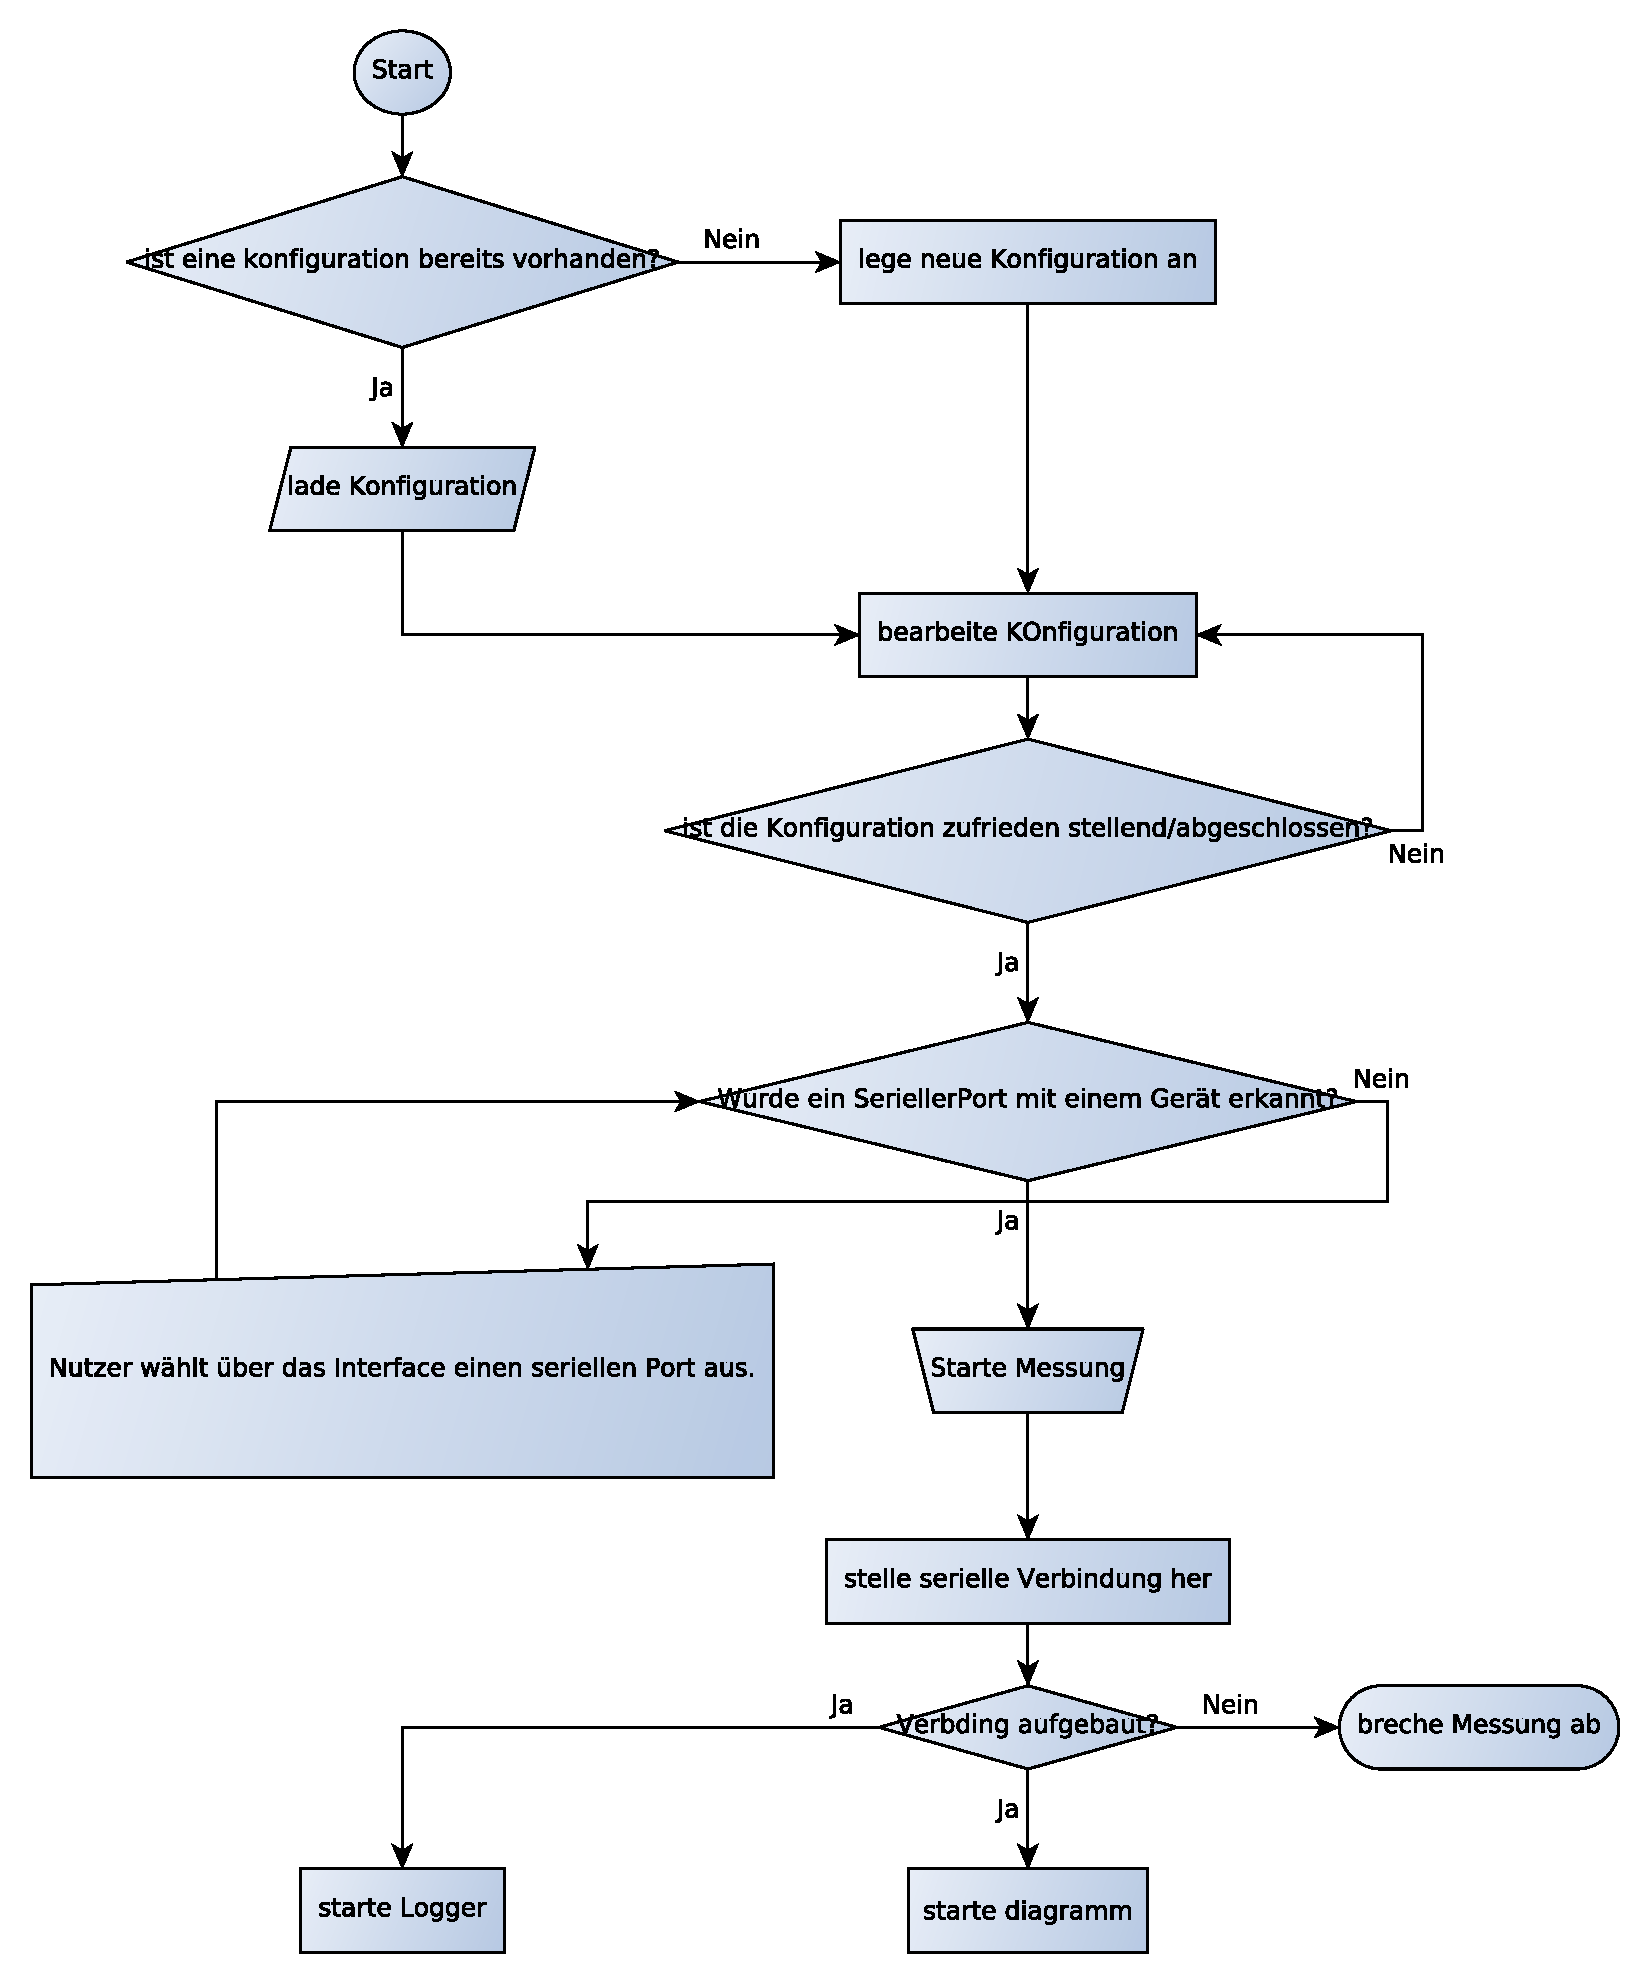
\includegraphics[width=\textwidth, keepaspectratio=true]{../Diagramme/SoftwareFlowChart.pdf}
\end{figure}
%\section{Aufbau}
%grobes UML
%\section{User Interface - Wireframe}